\def\mytitle{FPGA Assignment}
\def\myauthor{Naru Soundarya}
\def\contact{narusoundarya2002@gmail.com}
\def\mymodule{Future Wireless Communication (FWC)}
\documentclass[10pt, a4paper]{article}
\usepackage[a4paper,outer=1.5cm,inner=1.5cm,top=1.75cm,bottom=1.5cm]{geometry}
\twocolumn
\usepackage{setspace}
\usepackage{graphicx}
\graphicspath{{./images/}}
\usepackage[colorlinks,linkcolor={black},citecolor={blue!80!black},urlcolor={blue!80!black}]{hyperref}
\usepackage[parfill]{parskip}
\usepackage{lmodern}
\usepackage{tikz}
	\usepackage{physics}
%\documentclass[tikz, border=2mm]{standalone}
\usepackage{karnaugh-map}
\usepackage{tabularx}
\usetikzlibrary{calc}
\usepackage{amsmath}
\usepackage{amssymb}
\renewcommand*\familydefault{\sfdefault}
\usepackage{watermark}
\usepackage{lipsum}
\usepackage{xcolor}
\usepackage{listings}
\usepackage{float}
\usepackage{titlesec}
\providecommand{\mtx}[1]{\mathbf{#1}}
\titlespacing{\subsection}{1pt}{\parskip}{3pt}
\titlespacing{\subsubsection}{0pt}{\parskip}{-\parskip}
\titlespacing{\paragraph}{0pt}{\parskip}{\parskip}

\newcommand{\myvec}[1]{\ensuremath{\begin{pmatrix}#1\end{pmatrix}}}
\let\vec\mathbf
\lstset{
frame=single, 
breaklines=true,
columns=fullflexible
}
\title{\mytitle}
\author{\myauthor\hspace{1em}\\\contact\\FWC22021\hspace{6.5em}IITH\hspace{0.5em}\mymodule\hspace{6em}ASSIGN}
\date{}

\begin{document}
	\maketitle
\section{Problem}
 Write the Boolean Expression for the result of the Logic Circuit as shown below:
\begin{figure}[h]
    \centering
    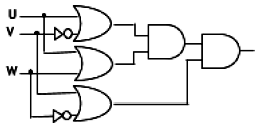
\includegraphics[scale=1]{1.PNG}
     \caption{circuit}
      \label{fig:circuit}
\end{figure}
\section{solution}
    %\caption
    \begin{center}
    	${\boldsymbol{F}=\boldsymbol{U}(\boldsymbol{V}+\boldsymbol{!W})}$
    \end{center}

\section{Components}
  \begin{tabularx}{0.4\textwidth} { 
  | >{\centering\arraybackslash}X 
  | >{\centering\arraybackslash}X 
  | >{\centering\arraybackslash}X | }
\hline
 \textbf{Components}& \textbf{Values} & \textbf{Quantity}\\
\hline
Vaman &  & 1 \\  
\hline
JumperWires& M-F & 5 \\ 
\hline
Breadboard &  & 1 \\
\hline
USB-C cable&  & 1 \\
\hline
LED & & 1 \\
\hline
\end{tabularx}
   
\section{Setup}
\begin{enumerate}
\item Connect the Vaman to the Laptop through USB.
\item There is a button and an LED to the left of the USB port on the Vaman.There is another button to the right of the LED.
\item Press the right button first and immediately press the left button.The LED will be blinking green.The Vaman is now in bootloader mode.
\end{enumerate}
\subsection{Steps for implementation}
\begin{enumerate}
\item Login to termux-ubuntu on the android device and execute the following commands:\\
Make sure that the required installation and tool builds of pygmy-sdk had done prior executing below commands
\begin{lstlisting}
proot-distro login debian
cd  /data/data/com.termux/files/home/
mkdir fpga
svn co https://github.com/soundaryanaru/FWC-assignments/trunk/fpga/codes
cd codes
ql_symbiflow -compile -src /data/data/com.termux/files/home/fpga/codes -d ql-eos-s3 -P PU64 -v helloworldfpga.v -t helloworldfpga -p quickfeather.pcf -dump binary
\end{lstlisting}
This will generate \textbf{helloworldfpga.bin} file in codes directory transfer this bin file to laptop by executing the following command
\begin{lstlisting}
scp /data/data/com.termux/files/home/fpga/codes/helloworldfpga.bin username_of_pc@IP_address:/home/username
\end{lstlisting}
Make sure that the appropriate username,IP address of the Laptop is given in the above command.
\item Now execute the following commands on the Laptop terminal\\
Make sure that required installation of programmer application had done prior executing below command
\begin{lstlisting}
python3 /home/username/TinyFPGA-Programmer-Application/tinyfpga-programmer-gui.py --port /dev/ttyACM0 --appfpga /home/username/helloworldfpga.bin --mode fpga
\end{lstlisting}
\item After finishing the process of flashing with the programmer application press the button to the right of the USB port to reset. Vaman is now flashed with our source code
\end{enumerate}
\section{Implementation}
The code below realizes the Boolean logic for F   using 5V,GND of Vaman Board using Verilog Language
\begin{center}
\fbox{\parbox{8.5cm}{\url{https://github.com/soundaryanaru/FWC-assignments/blob/main/fpga/codes/helloworldfpga.v}}}
\end{center}
\end{document}
